%%%%%%%% ICML 2026 EXAMPLE LATEX SUBMISSION FILE %%%%%%%%%%%%%%%%%

\documentclass{article}

% Recommended, but optional, packages for figures and better typesetting:
\usepackage{microtype}
\usepackage{graphicx}
\usepackage{subcaption}
\usepackage{booktabs} % for professional tables
\usepackage{listings}
\usepackage{xcolor} % optional, for syntax highlighting
\usepackage{float} % for H placement
\usepackage{tikz}
\usepackage{tabularx}
\usetikzlibrary{arrows.meta, positioning, decorations.pathreplacing}

\usepackage{tcolorbox}   % for boxed listings
\tcbset{
    mypythonbox/.style={
        listing engine=listings,
        listing only,
        breakable,
        enhanced,
        colback=gray!5,
        colframe=black,
        boxrule=0.5pt,
        arc=2mm,
        outer arc=2mm,
        left=2mm,
        right=2mm,
        top=1mm,
        bottom=1mm,
        title=#1,
    }
}

% Optional: configure listings for Python
\lstset{
    language=Python,
    basicstyle=\ttfamily\small,
    keywordstyle=\color{blue},
    stringstyle=\color{red!70!black},
    commentstyle=\color{green!50!black},
    numbers=left,
    numberstyle=\tiny,
    stepnumber=1,
    numbersep=5pt,
    breaklines=true,
    showstringspaces=false
}


% hyperref makes hyperlinks in the resulting PDF.
% If your build breaks (sometimes temporarily if a hyperlink spans a page)
% please comment out the following usepackage line and replace
% \usepackage{icml2026} with \usepackage[nohyperref]{icml2026} above.
\usepackage{hyperref}


% Attempt to make hyperref and algorithmic work together better:
\newcommand{\theHalgorithm}{\arabic{algorithm}}

% Use the following line for the initial blind version submitted for review:
\usepackage{icml2026}

% For preprint, use
% \usepackage[preprint]{icml2026}

% If accepted, instead use the following line for the camera-ready submission:
% \usepackage[accepted]{icml2026}

\usepackage{amsmath}
\usepackage{amssymb}
\usepackage{mathtools}
\usepackage{amsthm}


% if you use cleveref..
\usepackage[capitalize,noabbrev]{cleveref}

%%%%%%%%%%%%%%%%%%%%%%%%%%%%%%%%
% THEOREMS
%%%%%%%%%%%%%%%%%%%%%%%%%%%%%%%%
\theoremstyle{plain}
\newtheorem{theorem}{Theorem}[section]
\newtheorem{proposition}[theorem]{Proposition}
\newtheorem{lemma}[theorem]{Lemma}
\newtheorem{corollary}[theorem]{Corollary}
\theoremstyle{definition}
\newtheorem{definition}[theorem]{Definition}
\newtheorem{assumption}[theorem]{Assumption}
\theoremstyle{remark}
\newtheorem{remark}[theorem]{Remark}

% Todonotes is useful during development; simply uncomment the next line
%    and comment out the line below the next line to turn off comments
%\usepackage[disable,textsize=tiny]{todonotes}
\usepackage[textsize=tiny]{todonotes}

% The \icmltitle you define below is probably too long as a header.
% Therefore, a short form for the running title is supplied here:
\icmltitlerunning{Hardware-Aware Reformulation of CNNs for Efficient Execution on Specialized AI Hardware}


\begin{document}

\twocolumn[
	\icmltitle{Hardware-Aware Reformulation of CNNs for Efficient Execution on Specialized AI Hardware: A Case Study on NVIDIA Tensor Cores}


  % It is OKAY to include author information, even for blind submissions: the
  % style file will automatically remove it for you unless you've provided
  % the [accepted] option to the icml2026 package.

  % List of affiliations: The first argument should be a (short) identifier you
  % will use later to specify author affiliations Academic affiliations
  % should list Department, University, City, Region, Country Industry
  % affiliations should list Company, City, Region, Country

  % You can specify symbols, otherwise they are numbered in order. Ideally, you
  % should not use this facility. Affiliations will be numbered in order of
  % appearance and this is the preferred way.
  \icmlsetsymbol{equal}{*}

  \begin{icmlauthorlist}
    \icmlauthor{Firstname1 Lastname1}{equal,yyy}
  \end{icmlauthorlist}

  % You may provide any keywords that you find helpful for describing your
  % paper; these are used to populate the "keywords" metadata in the PDF but
  % will not be shown in the document
  \icmlkeywords{Machine Learning, ICML}

  \vskip 0.3in
]

\begin{abstract}
	Convolutional Neural Networks (CNNs) are central to modern AI, but their performance is often limited by hardware constraints. NVIDIA Tensor Cores, for instance, require input channels to be multiples of 8 for efficient execution. Traditional approaches address such alignment using zero-padding, which can be inefficient. In this work, we present a first-step, hardware-aware reformulation of CNN computations using rewrite rules, restructuring the underlying math to satisfy hardware alignment entirely {\bf post-training} without modifying network weights. While our current implementation focuses on a single transformation for Tensor Cores, this approach is generalizable, laying the foundation to explore additional transformations for other accelerators, including AMD GPUs. This study represents an initial step toward {\em semantic tuning}, a systematic, hardware-aware optimization strategy for efficient deployment of CNN models on specialized AI hardware.
\end{abstract}

\section{Introduction}

Convolutional Neural Networks (CNNs) are a foundational building block of modern deep learning systems, underpinning applications ranging from computer vision to speech and scientific computing. At a high level, CNNs apply learnable filters to structured input tensors in order to extract hierarchical feature representations. For a standard convolution, the input tensor has shape $(B, C_{\text{in}}, H[, W, D])$, the filter weights have shape $(C_{\text{out}}, C_{\text{in}}, K_1[, K_2, \ldots, K_n])$, and the resulting output tensor has shape $(B, C_{\text{out}}, H_{\text{out}}[, W_{\text{out}}, D_{\text{out}])}$.

While this mathematical formulation is hardware-agnostic, the efficient execution of CNNs on modern AI accelerators is strongly influenced by hardware-specific constraints. Specialized units such as NVIDIA Tensor Cores and analogous matrix-multiply engines in other accelerators impose alignment and tiling requirements on tensor dimensions, most notably that certain dimensions (e.g., channel counts) be multiples of fixed factors such as eight~\cite{nvidia_cnn}. When these constraints are not satisfied, accelerators either fall back to less efficient execution paths or require auxiliary modifications such as zero padding, which introduce redundant computation and memory overhead.

Existing approaches typically address these constraints during network design or training, for example by manually choosing channel dimensions or retraining models with padded tensors. In contrast, this paper explores a complementary and largely underexplored direction: post-training reformulation of CNN computations. Rather than modifying the network architecture or retraining weights, we rewrite the underlying convolutional mathematics to produce an equivalent formulation that satisfies hardware alignment requirements by construction.

Specifically, we present an initial hardware-aware transformation that reshapes and reinterprets the convolutional computation—through {\bf width folding} and {\bf structured filter expansion} —so that the resulting tensors conform to accelerator alignment constraints while preserving exact numerical equivalence to the original CNN. This transformation eliminates the need for zero padding and does not alter the learned parameters or outputs of the network. Although the paper focuses on a single transformation motivated by NVIDIA Tensor Core constraints, the broader goal is to establish a foundation for a family of such rewrite rules that can be systematically derived and applied across different accelerator architectures.

Viewed through this lens, CNN execution can be treated as a compilation problem, where mathematically equivalent reformulations are selected to best match the capabilities and constraints of the target hardware. This work represents a first step toward such a hardware-aware compilation framework for CNNs, demonstrating that non-trivial accelerator constraints can be addressed purely through post-training mathematical rewrites.

%\begin{figure}[h!]
%    \centering
%    \includegraphics[width=0.8\columnwidth]{scheme4.png}
%    \caption{Illustration of the block-diagonal filter transformation for a 1-D CNN. The input tensor is reshaped and combined with a block-diagonal filter to produce a Tensor Core-efficient output.}
%    \label{fig:blockdiag1d}
%\end{figure}

%\onecolumn
\begin{figure}[h!]
\centering
\resizebox{\columnwidth}{!}{%
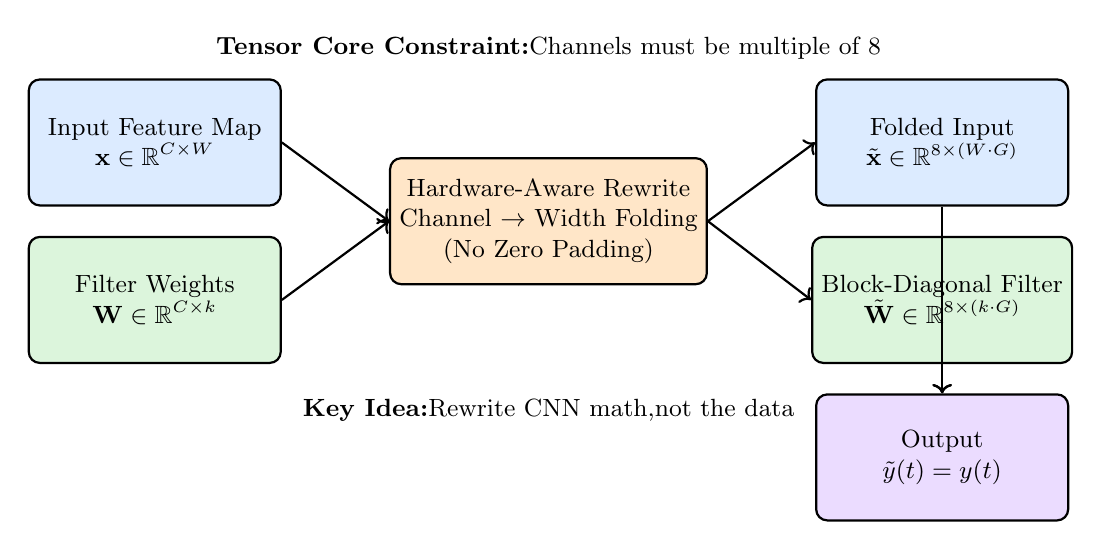
\begin{tikzpicture}[
    box/.style={draw, thick, rounded corners, minimum width=3.2cm, minimum height=1.6cm, align=center},
    arrow/.style={->, thick},
    every node/.style={font=\small}
]

% Colors
\definecolor{inputblue}{RGB}{220,235,255}
\definecolor{filtergreen}{RGB}{220,245,220}
\definecolor{rewriteorange}{RGB}{255,230,200}
\definecolor{outputpurple}{RGB}{235,220,255}

% Original CNN
\node[box, fill=inputblue] (input1) at (0,2)
{Input Feature Map\\
$\mathbf{x} \in \mathbb{R}^{C \times W}$};

\node[box, fill=filtergreen] (filter1) at (0,0)
{Filter Weights\\
$\mathbf{W} \in \mathbb{R}^{C \times k}$};

% Rewrite
\node[box, fill=rewriteorange] (rewrite) at (5,1)
{Hardware-Aware Rewrite\\
Channel $\rightarrow$ Width Folding\\
(No Zero Padding)};

% New CNN
\node[box, fill=inputblue] (input2) at (10,2)
{Folded Input\\
$\tilde{\mathbf{x}} \in \mathbb{R}^{8 \times (W \cdot G)}$};

\node[box, fill=filtergreen] (filter2) at (10,0)
{Block-Diagonal Filter\\
$\tilde{\mathbf{W}} \in \mathbb{R}^{8 \times (k \cdot G)}$};

% Output
\node[box, fill=outputpurple] (output) at (10,-2)
{Output\\
$\tilde{y}(t) = y(t)$};

% Arrows
\draw[arrow] (input1.east) -- (rewrite.west);
\draw[arrow] (filter1.east) -- (rewrite.west);

\draw[arrow] (rewrite.east) -- (input2.west);
\draw[arrow] (rewrite.east) -- (filter2.west);

\draw[arrow] (input2.south) -- (output.north);
\draw[arrow] (filter2.south) -- (output.north);

% Annotation
\node at (5,3.2)
{\textbf{Tensor Core Constraint:}\\
Channels must be multiple of 8};

\node at (5,-1.4)
{\textbf{Key Idea:}\\
Rewrite CNN math,\\
not the data};

\end{tikzpicture}
}
\caption{Hardware-aware reformulation of a CNN via channel-to-width folding.
The rewrite preserves exact semantics while satisfying Tensor Core alignment
constraints without zero padding or retraining.}

\label{fig:cnn_rewrite}
\end{figure}


\begin{figure}[t]
\centering
\resizebox{\columnwidth}{!}{%
\begin{tikzpicture}[font=\small]

% =========================
% Styles (ALL IN ONE BLOCK)
% =========================
\tikzset{
    tensor/.style={
        draw,
        thick,
        rounded corners=2pt,
        top color=#1!20,
        bottom color=#1!60,
        shading angle=45
    },
    depth/.style={
        draw,
        thick,
        fill=#1!40,
        opacity=0.85
    },
    kernel3d/.style={
        draw,
        thick,
        left color=gray!20,
        right color=gray!60
    },
    cell/.style={
        draw,
        thick,
        fill=gray!12
    },
    diag/.style={
        draw,
        thick,
        fill=red!65,
        drop shadow
    },
    arrow/.style={
        ->,
        thick,
        color=blue!70
    }
}

% =========================
% Original Input Tensor (H x W, C=1)
% =========================
\node[tensor=blue, minimum height=2.2cm, minimum width=4.2cm] (orig) at (0,0) {};
%\node[depth=blue, minimum height=2.2cm, minimum width=4.2cm] at (0.15,0.15) {};
\node[above=4pt of orig] {Input tensor};
\node[below=4pt of orig] {$H \times W,\; C_{in}=1$};

% =========================
% Width Folding Arrow
% =========================
\draw[arrow] (orig.east) to[out=0,in=180] ++(1.6,0)
node[midway,above] {Width folding ($F=8$)};

% =========================
% Folded Input (Channel Depth = 8)
% =========================
\begin{scope}[shift={(6,0)}]
    \foreach \i/\c in {
        0/red,
        1/orange,
        2/yellow,
        3/green,
        4/cyan,
        5/blue,
        6/purple,
        7/magenta
    } {
        \node[depth=\c, minimum height=2.2cm, minimum width=0.6cm]
        at (\i*0.18, \i*0.18) {};
    }

    \node at (1.6,1.9) {Folded input};
    \node at (1.6,-1.5) {$H \times (W/8)$};
    \node at (1.6,-2.1) {$C_{in}' = 8$};
    \node[align=center] at (1.6,-2.8)
        {\scriptsize Channels stacked in depth};
\end{scope}

% =========================
% Original Filter
% =========================
\begin{scope}[shift={(0,-4.8)}]
    \node[kernel3d, minimum width=0.45cm, minimum height=2.2cm] (filt) at (0,0) {};
    \node[above=4pt of filt] {Original filter};
    \node[below=4pt of filt] {$K \times 1$};
\end{scope}

% =========================
% Filter Expansion Arrow
% =========================
\draw[arrow] (1.1,-4.8) to[out=0,in=180] (2.6,-4.8)
node[0.5,above] {Channel expansion};

% =========================
% Expanded Diagonal Filter (8 x 8)
% =========================
\begin{scope}[shift={(5.2,-6.6)}, yscale=-1]
    % Shadow (3D effect)
    \begin{scope}[opacity=0.15]
        \foreach \i in {0,...,7} {
            \foreach \j in {0,...,7} {
                \node[cell, fill=black]
                at (\j*0.5+0.08, \i*0.5+0.08) {};
            }
        }
    \end{scope}

    % Main grid
    \foreach \i in {0,...,7} {
        \foreach \j in {0,...,7} {
            \ifnum\j=\i
                \node[cell,diag] at (\j*0.5, \i*0.5) {};
            \else
                \node[cell] at (\j*0.5, \i*0.5) {};
            \fi
        }
    }

    \node at (1.75,4.3) {Expanded filter};
    \node at (1.75,-1.1) {Diagonal replication};
    \node at (1.75,-1.7) {$C_{in}' = 8$};
\end{scope}

\end{tikzpicture}
}
\caption{
Semantic-preserving CNN reformulation via width folding.
The input width is partitioned into $F=8$ interleaved slices and stacked along the channel dimension, increasing the effective number of input channels without altering spatial height.
The original $K \times 1$ convolution kernel is replicated along the main diagonal of the expanded filter matrix, ensuring independent convolution of each folded slice.
This post-training transformation preserves exact convolution semantics while aligning channel dimensions with accelerator constraints.
}
\label{fig:full-width-folding}
\end{figure}


%\clearpage       % start on a fresh page
%\onecolumn

\section{Width Folding Transformation}

This section describes the width folding transformation, a post-training,
semantics-preserving reformulation that increases the effective channel
dimension to satisfy hardware alignment constraints while leaving the learned
model parameters unchanged.

Given an input tensor
\[
X \in \mathbb{R}^{H \times W \times C_{in}}, \quad C_{in}=1,
\]
and a 1-D convolution kernel
\[
W_f \in \mathbb{R}^{K \times 1},
\]
we fold the width dimension by a factor $F$ such that $W$ is divisible by $F$.
The transformation produces an equivalent convolution with
\[
C_{in}' = F, \quad W' = W / F,
\]
while preserving exact convolution semantics.

\subsection{Input Width Folding}

The width folding operation partitions the width dimension into $F$ interleaved
slices and stacks them along the channel dimension.
Formally, the transformed input tensor
\[
X' \in \mathbb{R}^{H \times (W/F) \times F}
\]
is defined as
\begin{equation}
X'(h, w', f) = X(h, Fw' + f),
\quad
f = 0,\ldots,F-1.
\label{eq:width_fold_def}
\end{equation}

This operation is a pure re-indexing and does not alter the numerical values of
the input tensor.

\subsection{Filter Construction}

Because convolution is performed only along the height dimension, each width
slice is convolved independently.
To preserve this behavior after folding, the original filter is replicated
across the expanded channel dimension without introducing cross-channel mixing.

Let the original filter be
\[
W_f \in \mathbb{R}^{K \times 1}.
\]
We construct a new filter tensor
\[
W_f' \in \mathbb{R}^{K \times F \times F}
\]
as a diagonal replication:
\begin{equation}
W_f'(k, f, f')
=
\begin{cases}
W_f(k), & f = f', \\
0, & f \neq f'.
\end{cases}
\label{eq:filter_construct}
\end{equation}

In implementation terms, this corresponds to allocating a zero-initialized
filter tensor and copying the original filter into the diagonal channel blocks.
Conceptually, each folded width slice receives an identical copy of the
original kernel.

\subsection{Bias Construction}

The original convolution bias
\[
b \in \mathbb{R}
\]
is shared across all folded slices.
Accordingly, the new bias vector is constructed by replication:
\begin{equation}
b'(f) = b,
\quad
f = 0,\ldots,F-1.
\label{eq:bias_construct}
\end{equation}

This ensures that each expanded channel applies the same bias as in the
original formulation.

\subsection{Resulting Convolution}

After width folding and filter construction, the transformed convolution
operates on
\[
X' \in \mathbb{R}^{H \times (W/F) \times F}
\]
using the filter $W_f'$ and bias $b'$.
As shown in Section~\ref{sec:correctness}, this convolution produces outputs
that are exactly equivalent to those of the original network, up to a
bijective re-indexing of the width dimension.


\section{Correctness of Width Folding Transformation}

We consider a 1-D convolution performed exclusively along the height
dimension \(H\).
The width dimension \(W\) does not participate in the convolution and is
treated as an independent indexing dimension.

Let the input tensor be
\[
X \in \mathbb{R}^{H \times W \times C_{in}}, \quad C_{in} = 1,
\]
and let the convolution filter be
\[
W_f \in \mathbb{R}^{K \times 1},
\]
with bias \(b \in \mathbb{R}\).
Batch and output channel indices are omitted for clarity.

The original convolution output is given by
\begin{equation}
Y(h, w)
=
\sum_{k=0}^{K-1}
W_f(k)\, X(h+k, w) + b,
\label{eq:orig_conv_H}
\end{equation}
where convolution is performed only along the height dimension.

\paragraph{Width Folding Transformation.}
Let \(F\) be the folding factor and assume \(W\) is divisible by \(F\).
We define a transformed input tensor
\[
X' \in \mathbb{R}^{H \times (W/F) \times F}
\]
by re-indexing the width dimension as
\begin{equation}
X'(h, w', f)
=
X(h, Fw' + f),
\quad
f = 0,\ldots,F-1.
\label{eq:width_fold}
\end{equation}
This operation folds the width dimension into the channel dimension
without modifying spatial data along \(H\).

\paragraph{Filter Expansion.}
Since the convolution is independent across width indices, the filter
must be replicated for each folded slice.
We define an expanded filter
\[
W_f' \in \mathbb{R}^{K \times F \times F}
\]
as a diagonal replication:
\begin{equation}
W_f'(k, f, f')
=
\begin{cases}
W_f(k), & f = f', \\
0, & f \neq f'.
\end{cases}
\label{eq:diag_filter_H}
\end{equation}
The bias is similarly replicated as \(b'(f) = b\).

\paragraph{Transformed Convolution.}
The output of the transformed convolution is
\begin{equation}
Y'(h, w', f)
=
\sum_{k=0}^{K-1}
\sum_{f'=0}^{F-1}
W_f'(k,f,f')\, X'(h+k, w', f')
+ b'(f).
\label{eq:new_conv_H}
\end{equation}

Substituting Eq.~\eqref{eq:diag_filter_H} into
Eq.~\eqref{eq:new_conv_H} removes the channel summation:
\begin{equation}
Y'(h, w', f)
=
\sum_{k=0}^{K-1}
W_f(k)\, X'(h+k, w', f) + b.
\label{eq:new_conv_simplified_H}
\end{equation}

Using the folded input definition from
Eq.~\eqref{eq:width_fold}, we obtain
\[
Y'(h, w', f)
=
\sum_{k=0}^{K-1}
W_f(k)\, X(h+k, Fw' + f) + b.
\]

Let \(w = Fw' + f\).
Then
\[
Y'(h, w', f) = Y(h, w),
\]
where \(Y(h,w)\) is the output of the original convolution defined in
Eq.~\eqref{eq:orig_conv_H}.

\paragraph{Conclusion.}
The width folding transformation constitutes a bijective re-indexing of
the width dimension combined with diagonal filter replication.
Since the convolution is performed solely along the height dimension,
the transformation preserves the exact numerical output of the original
network.
Therefore, width folding with channel expansion is
\emph{semantics preserving}.
\hfill\(\square\)

\subsection{N-D Convolutions}
Our method generalizes to N-D convolutions by folding dimensions that are not involved in the convolution operation into the channel dimension. This reparameterization preserves exact convolution semantics via block-diagonal kernels and does not rely on kernel separability or approximation.
%\vspace{2mm} % small spacing between figure and code

\section{Survey of Popular CNN Architectures}
To motivate the need for hardware-aware filter alignment, we survey several widely used CNN architectures and their first-layer channel dimensions. Many modern networks have input channel dimensions that are not multiples of 8, which can lead to underutilization of NVIDIA Tensor Cores.
\begin{table}[h!]
\centering
\small
\caption{First-layer channels in popular CNN architectures}
\label{tab:firstlayer}
\begin{tabularx}{\columnwidth}{|X|c|c|X|}
\hline
\textbf{Network} & \textbf{Input Channels} & \textbf{First Conv Filters} & \textbf{Notes} \\
\hline
AlexNet  & 3 & 96 & RGB input \\
VGG16  & 3 & 64 & RGB input \\
ResNet-18 & 3 & 64 & RGB input \\
ResNet-50 & 3 & 64 & RGB input \\
GoogLeNet & 3 & 64 & RGB input \\
MobileNetV2 & 3 & 32 & RGB input \\
\hline
\end{tabularx}
\end{table}

As shown in Table~\ref{tab:firstlayer}, most models processing RGB images have an input channel count of 3, which is not a multiple of 8, limiting the efficiency on NVIDIA Tensor Cores. This motivates the use of padding or block-diagonal transformations to maximize hardware throughput. Proprietary networks with similar input channels could benefit from the same approach. Furthermore, many models have a first-layer filter count below 512, which is the optimal number recommended by NVIDIA~\cite{nvidia_cnn}. In such cases, our method can also increase the channel dimensions, ensuring better alignment with hardware requirements while preserving network functionality.

\section{Potential Optimizations for Sparsity}
Efficient exploitation of sparsity is crucial for both memory savings and computational acceleration. The block-diagonal filter structure introduces structured sparsity that can be leveraged in multiple ways:

\begin{itemize}
    \item \textbf{Memory:} Only the diagonal blocks of the filters contain non-zero values, while off-diagonal blocks are zero. This structured sparsity allows storing just the non-zero blocks in memory as sparse tensors, significantly reducing memory footprint. For large networks, this can lead to substantial savings, especially in embedded or GPU-constrained environments.
    
    \item \textbf{Computation:} Convolutions involving zero blocks do not contribute to the output, so these computations can be safely skipped. Modern deep learning frameworks and custom CUDA kernels can exploit this by performing sparse matrix multiplications, reducing the number of operations and increasing throughput.
    
    \item \textbf{Framework Support:} Popular deep learning frameworks such as PyTorch and TensorFlow provide built-in support for grouped and sparse convolutions. By mapping each diagonal block to a group, the block-diagonal convolution can be implemented efficiently without modifying the core framework. Additionally, frameworks may optimize memory access patterns to reduce cache misses during sparse computations.
    
    \item \textbf{Quantization:} Structured sparsity pairs naturally with mixed-precision quantization (FP16/INT8). By representing both weights and activations in lower precision, memory bandwidth is reduced, and Tensor Cores can achieve higher throughput. Combining quantization with block-diagonal sparsity ensures that only essential computations are performed at high speed, improving overall efficiency while maintaining model accuracy.
\end{itemize}

\section {Extending the transformation}
Table~\ref{tab:cnn_transformations} summarizes a set of potential hardware-aware CNN transformations that extend the core idea explored in this work. While the width folding transform itself was derived manually from first principles, the transformations in Table~\ref{tab:cnn_transformations} were generated by AI (ChatGPT). All transformations are post-training and operate by rewriting the underlying convolutional computation to satisfy hardware-specific alignment and execution constraints, rather than relying on conventional techniques such as zero padding or network retraining. The transformations are ordered by increasing conceptual and implementation complexity, ranging from simple channel and spatial folding to more advanced sparsity-aware and N-dimensional rewrites. While only a single transformation is formally derived and validated in this paper, the table outlines a broader design space of mathematically equivalent reformulations that could be systematically explored in future work. These transformations are currently unverified and are intended to illustrate how a rule-based or compiler-driven framework could generalize the proposed approach across different accelerator architectures, including but not limited to NVIDIA Tensor Cores.


\begin{table*}[t]
\centering
\small
\caption{Potential (unverified) hardware-aware CNN transformations (post-training), generated by AI.}
\label{tab:cnn_transformations}
\begin{tabularx}{\textwidth}{|l|X|X|X|}
\hline
\textbf{Transformation} & \textbf{Description} & \textbf{Hardware Constraint Addressed} & \textbf{Notes / Benefits} \\
\hline
Kernel Reordering / Permutation & Reorder kernel elements to match hardware memory layout & Memory coalescing, tensor core tiling & Improves cache utilization \\
Depthwise / Grouped Splitting & Split convolution into depthwise or grouped operations & SIMD or tensor-core efficiency & Increases parallelism \\
Spatial Folding / Height Folding & Fold spatial dimensions to match tile sizes & Vector-width alignment & Useful for large images \\
Precision Folding / Mixed-Precision Rewriting & Convert weights/activations to FP16 or BF16 & Tensor core precision constraints & Improves throughput \\
Channel Pruning & Remove redundant channels and repack remaining ones & Channel alignment & Can combine with folding \\
Strided / Dilated Rewriting & Rewrite strided/dilated convolutions & Tile-size optimization & Preserves output equivalence \\
Sparsity-Aware Weight Folding & Rearrange sparse weights into dense aligned blocks & Block-sparse GEMM & Exploits structured sparsity \\
N-D Dimension Folding & Extend folding to 2D/3D convolutions & Multi-dimensional tiling & Generalizes channel folding \\
\hline
\end{tabularx}
\end{table*}
%\clearpage


%\twocolumn



\section{Related Work}
Optimizing CNNs for hardware accelerators has been an active area of research. \textit{NVIDIA Tensor Cores} and other mixed-precision matrix multiplication units benefit from channel alignment~\cite{micikevicius2017mixed}. Previous work on grouped~\cite{krizhevsky2012imagenet} and depthwise convolutions~\cite{howard2017mobilenets} introduces structured sparsity for efficiency. Our approach draws inspiration from these techniques, combining channel expansion and block-diagonal sparsity to fully exploit hardware throughput. Similar strategies have been explored in low-rank filter approximations~\cite{jaderberg2014speeding} and kernel tiling optimizations~\cite{chetlur2014cudnn}, but our method maintains the original filter semantics while providing full Tensor Core alignment.

\subsection{Relation to Other CNN Variants}

\subsubsection{Grouped Convolutions}
In grouped convolutions, input channels are divided into separate groups, and each group is convolved independently with a corresponding set of filters. Our block-diagonal transformation naturally induces a similar structure: each diagonal block in the filter corresponds to a “group” that processes a subset of the input channels. However, unlike standard grouped convolutions, our approach preserves the original filter values within each block and replicates them in a controlled manner to align with Tensor Core hardware. This ensures maximum hardware utilization without changing the semantic meaning of the original convolution.

\subsubsection{Depthwise and Pointwise Convolutions}
Depthwise convolutions apply a single filter per input channel, significantly reducing computation but also limiting feature interactions across channels. Pointwise (1×1) convolutions are then used to combine features across channels. The block-diagonal filter transformation resembles a hybrid of these approaches: each block is multi-channel (not single-channel as in depthwise) and operates on a subset of input channels, while off-diagonal blocks are zeroed to create structured sparsity. This design maintains full multi-channel processing within blocks while still enabling computational efficiency similar to depthwise convolutions. Unlike traditional depthwise or pointwise convolutions, our method explicitly targets hardware alignment for Tensor Cores.

\subsubsection{Channel Expansion / 1×1 Convolutions}
Channel expansion via 1×1 convolutions is commonly used to increase the number of output channels and enable more expressive representations. In our approach, the block-diagonal transformation can be interpreted as a structured channel expansion: the original output channels are replicated across diagonal blocks to create a padded, hardware-aligned output tensor. This provides the benefits of channel expansion—higher representational capacity—without introducing additional learnable parameters beyond the original filter. The key distinction is that our expansion is carefully organized to match hardware constraints, which is not considered in conventional 1×1 convolutions.

\subsection{Difference from Channel Zero-Padding}

A naive approach to align channels for hardware efficiency is zero-padding in the channel dimension. For example, if a layer has 5 input channels and the hardware prefers multiples of 8, you could append 3 extra channels filled with zeros. While this ensures that the total number of channels is divisible by 8, it has several limitations:
\begin{itemize}
\item No reuse of original filter weights:
Zero-padding simply adds empty channels. The convolution computation over these extra channels does nothing useful—these channels carry no information.

\item Underutilized computation:
Even though the number of channels is aligned, Tensor Cores may still process these zero channels, wasting compute cycles on irrelevant data.

\item No structured sparsity for efficiency:
Channel zero-padding does not create a predictable pattern that frameworks can exploit. In contrast, block-diagonal filters introduce structured sparsity, where off-diagonal blocks are zero but the diagonal blocks contain actual filter weights. Frameworks can leverage this for efficient computation (skipping zeros).

\item Preserves semantic connections:
With channel zero-padding, the output channels corresponding to padded zeros produce meaningless feature maps. In contrast, the block-diagonal approach replicates the original filters across diagonal blocks, maintaining meaningful convolutional connections and expanding output channels in a controlled manner.

\item Better generalization to grouped and n-dimensional convolutions:
Block-diagonal filters naturally generalize to higher dimensions and grouped structures, while zero-padded channels remain sparse and unused, limiting flexibility and efficiency.
\end{itemize}

\section{Advantages of the Method}
The proposed block-diagonal filter transformation offers multiple advantages:
\begin{enumerate}
    \item \textbf{Hardware-aligned computation:} By padding and reorganizing channels, the method fully leverages Tensor Core throughput without modifying the underlying kernel operations.
    \item \textbf{Preservation of filter semantics:} The original filter patterns are maintained within diagonal blocks, ensuring that learned features and connectivity are preserved.
    \item \textbf{Structured sparsity:} Zero-filled off-diagonal blocks create structured sparsity, which can be exploited for memory and compute efficiency in modern deep learning frameworks.
    \item \textbf{Generalizability:} The approach extends naturally to 2-D, 3-D, and n-D convolutions, making it applicable to image, video, and volumetric data.
    \item \textbf{Compatibility:} Integrates seamlessly with existing CNN frameworks such as PyTorch and TensorFlow, allowing direct deployment on GPUs with Tensor Core support.
    \item \textbf{Reduced memory footprint:} Only diagonal blocks need to be stored densely, and sparse representations reduce memory usage.
    \item \textbf{Optimization potential with quantization:} Combining structured sparsity with mixed-precision operations (FP16/INT8) further improves throughput while maintaining accuracy.
    \item \textbf{Relationship to other convolution types:} Analogous to grouped, depthwise, and channel-expansion convolutions, it enables flexibility for designing efficient CNN architectures while maintaining high hardware utilization.
\end{enumerate}

\subsection{Contrast with Compiler Transformations}

Width folding differs fundamentally from conventional compiler
transformations applied in deep learning systems.
Traditional compiler optimizations—such as operator fusion, loop tiling,
layout reordering, vectorization, and kernel selection—preserve the
\emph{high-level mathematical definition} of an operator and optimize
\emph{how} that computation is executed on hardware.
These transformations act on scheduling, memory access patterns, or code
generation, but do not alter the underlying convolution formulation.

In contrast, width folding operates at the level of the \emph{mathematical
operator itself}.
The transformation explicitly rewrites the convolution into an equivalent
form by re-indexing tensor dimensions and restructuring filter parameters.
This reformulation changes the apparent tensor shapes and filter structure
seen by the compiler, while preserving exact input--output semantics by
construction.
As a result, hardware alignment constraints (e.g., channel dimensions being
multiples of a fixed factor) are satisfied without relying on padding or
special-case kernel implementations.

Another key distinction is the point at which the transformation is applied.
Compiler transformations are typically applied dynamically or at
compile time and are constrained by the original operator definitions
exposed in the computation graph.
Width folding is a \emph{post-training, pre-compilation} transformation:
it modifies the trained model itself before it is handed to the compiler or
runtime.
This enables downstream compilers to treat the transformed model as a
standard convolution that naturally maps to optimized hardware kernels.

Finally, while compiler transformations are generally opaque and
hardware-specific, width folding is expressed as an explicit, semantics-
preserving rewrite rule.
This makes the transformation analyzable, provably correct, and amenable to
future automation.
Rather than replacing compiler optimizations, width folding complements
them by expanding the space of hardware-friendly formulations that
compilers can further optimize.


\section{Results}
We implemented the proposed width transformation in both TensorFlow and cuDNN and validated it against standard, functionally equivalent convolution operations.  All experimental evaluations and ablation studies related to the width-folding transformation were conducted on NVIDIA A100 GPUs using proprietary CNN models. Due to intellectual property and data-sharing constraints, detailed experimental configurations, model architectures, and raw performance measurements cannot be publicly disclosed in this paper. The complete set of empirical results is therefore summarized in the accompanying patent application authored by the same author \cite{roche_pct}.

The reported results in the patent demonstrate up to $3\times$ performance improvement over baseline implementations on A100-class hardware, attributable to improved utilization of Tensor Cores through alignment-aware mathematical reformulation rather than conventional zero-padding strategies. H100 and B-series GPUs were not available at the time of experimentation.

This paper serves as a formal follow-up to the patent, providing a first-principles derivation, mathematical correctness proof, and generalization framework for the transformation. While the empirical results are documented elsewhere, the primary contribution here is the provably equivalent post-training reformulation of CNN computation, intended as a foundation for future automated and compiler-driven optimization efforts.
The observed results are consistent with publicly available documentation released by NVIDIA (NVIDIA Corporation, 2023). Furthermore, the proposed method is applicable to any convolutional layer—not limited to the first layer—and can also be extended to linear layers in deep neural networks, leading to even further speed up gains.

\section{Conclusion}
We presented a block-diagonal transformation for CNN filters that aligns input and output channels with NVIDIA Tensor Core requirements. The method maintains the original filter structure, generalizes to n-D convolutions, and exploits sparsity for memory and computational efficiency. This approach bridges hardware-aware optimizations with traditional CNN design principles, providing a practical and scalable solution for high-performance deep learning deployments.

\subsection{Future Work}

Several promising research directions follow naturally.
First, we plan to explore a broader class of \emph{structure-preserving
transformations} beyond block-diagonal reformulations. These include
alternative spatial--channel folding strategies, hierarchical blocking,
and mixed-radix reshaping schemes that may better match the execution
models of different accelerators. Such transformations could enable
efficient utilization of hardware units with strict alignment,
vectorization, or tiling requirements.

Second, while NVIDIA Tensor Cores motivated the current formulation,
the underlying idea is hardware-agnostic. Future work will investigate
transformations tailored to other GPU architectures, including AMD
GPUs, where wavefront sizes, memory coalescing rules, and matrix
instruction formats differ substantially. Developing a unified
transformation framework that adapts CNN operators to multiple
backends remains an open and important problem.

Third, we aim to extend these techniques to other operators commonly
used in modern architectures, such as depthwise separable convolutions,
attention mechanisms~\cite{attention}, and recurrent layers~\cite{lstm}. 
Identifying algebraic
equivalences that expose hardware-friendly structure without changing
model behavior could significantly broaden the impact of this approach.

Finally, we envision integrating these transformations into compiler and graph-optimization pipelines, such as TensorRT~\cite{tensorrt}. An alternative and complementary direction is to realize these transformations within an MLIR-based~\cite{mlir} compilation framework.  More broadly, we introduce \emph{semantic tuning} as a post-training optimization paradigm in which the mathematical formulation of a neural network is rewritten to better match hardware execution constraints while preserving the exact input–output semantics of the original model. Unlike traditional tuning techniques that modify network architectures, retrain parameters, or inject auxiliary operations such as zero padding, semantic tuning operates purely at the level of algebraic reformulation. The learned weights remain unchanged in value, and the network’s functional behavior is preserved by construction.

Overall, this work suggests a shift from hardware-specific kernel
optimization toward \emph{semantic operator transformations} as a
systematic method for achieving performance portability.

\bibliography{cnn_paper_icml}
\bibliographystyle{icml2026}

\newpage
\appendix
\onecolumn
% -----------------------------
% In your section where you want the figure
% -----------------------------
\section{Example Code using Tensorflow CNN (Channels-Last)}
This Tensorflow implementation demonstrates a 2-D block-diagonal filter transformation where the input is in **channels-last format** (`[B, H, W, C_in]`), the W dimension is folded, and the convolution is compatible with NVIDIA Tensor Cores.

\usepackage{listings}
\usepackage{xcolor}

\lstset{
    language=Python,
    basicstyle=\ttfamily\small,
    keywordstyle=\color{blue},
    commentstyle=\color{green!60!black},
    stringstyle=\color{orange},
    numbers=left,
    numberstyle=\tiny\color{gray},
    stepnumber=1,
    numbersep=5pt,
    showspaces=false,
    showstringspaces=false,
    breaklines=true,
    frame=single,
    caption={Width-folding CNN transformation in TensorFlow (channels-last).},
    label={lst:width_folding}
}

\begin{lstlisting}
import tensorflow as tf
import numpy as np

# -----------------------------
# Parameters
# -----------------------------
B, H, W = 1, 32, 64     # batch, height, width
K = 5                  # kernel size along H
F = 8                  # width folding factor
Cout = 1               # output channels

assert W % F == 0

# -----------------------------
# Input tensor (NHWC)
# -----------------------------
x = tf.random.normal((B, H, W, 1))

# -----------------------------
# Original filter + bias
# Conv along H only -> kernel (K,1)
# -----------------------------
filterVal = tf.random.normal((K, 1, 1, Cout))
biasVal = tf.random.normal((Cout,))

# -----------------------------
# Original convolution
# -----------------------------
y_orig = tf.nn.conv2d(
    x,
    filterVal,
    strides=[1, 1, 1, 1],
    padding="VALID",
    data_format="NHWC"
)
y_orig = tf.nn.bias_add(y_orig, biasVal)

# -----------------------------
# Width folding: W -> W/F, Cin -> F
# -----------------------------
# (B, H, W, 1) -> (B, H, W/F, F)
x_folded = tf.reshape(x, (B, H, W // F, F))

# -----------------------------
# Build diagonal filter
# (K,1,1,Cout) -> (K,1,F,F*Cout)
# -----------------------------
filterValNew = np.zeros((K, 1, F, F * Cout), dtype=np.float32)

for f in range(F):
    filterValNew[:, :, f, f*Cout:(f+1)*Cout] = np.squeeze(filterVal.numpy(),axis=-1)

filterValNew = tf.constant(filterValNew)

# -----------------------------
# Bias replication
# -----------------------------
biasValNew = tf.tile(biasVal, [F])

# -----------------------------
# Folded convolution
# -----------------------------
y_folded = tf.nn.conv2d(
    x_folded,
    filterValNew,
    strides=[1, 1, 1, 1],   # stride only along H
    padding="VALID",
    data_format="NHWC"
)
y_folded = tf.nn.bias_add(y_folded, biasValNew)

# -----------------------------
# Reconstruct original layout
# (B, H', W/F, F) -> (B, H', W)
# -----------------------------
y_reconstructed = tf.reshape(
    y_folded,
    (B, y_folded.shape[1], W)
)

# -----------------------------
# Verification
# -----------------------------
max_error = tf.reduce_max(tf.abs(np.squeeze(y_orig, axis=-1) - y_reconstructed))
print("Max absolute error:", max_error.numpy())

# Assert correctness
tf.debugging.assert_near(np.squeeze(y_orig, axis=-1), y_reconstructed, atol=1e-5)
print("✔ Width folding transformation is numerically correct")
\end{lstlisting}

\end{document}
